%%%%%%%%%%%%%%%%%%%%%%%%%%%%%%%%%%%%%%%%%%%%%%%%%%%%%%%%%%%%%%%%
% Template for BI-ZUM final report
% Encoding: UTF8
% Version: 1.0 (2013-01-28)
% Author: Ing. Martin Šlapák
%%%%%%%%%%%%%%%%%%%%%%%%%%%%%%%%%%%%%%%%%%%%%%%%%%%%%%%%%%%%%%%%
\documentclass[a4paper,10pt,twocolumn]{article}
\usepackage{lmodern}
\usepackage[english]{babel}
\usepackage[T1]{fontenc}
\usepackage[utf8]{inputenc}
\usepackage{amsfonts}
\usepackage{mathtools}
\usepackage{graphicx}
\usepackage{listings}
\usepackage{url}
\lstset{basicstyle=\normalfont\small,breaklines=true,columns=flexible}
\usepackage{float}
\usepackage[top=0.5cm,bottom=2cm,left=1cm,right=1cm]{geometry}

\usepackage{color}
\usepackage{xcolor}
\usepackage{listings}
\usepackage{caption}
\DeclareCaptionFont{white}{\color{white}}
\DeclareCaptionFormat{listing}{\colorbox{gray}{\parbox{0.4928\textwidth}{#1#2#3}}}
\captionsetup[lstlisting]{format=listing,labelfont=white,textfont=white,margin={-3.45pt,0pt}}
%%%%%%%%%%%%%%%%%%%%%%%%%%%%%%%%%%%%%%%%%%%%%%%%%%%%%%%%%%%%%%%%
% Source: http://tex.stackexchange.com/questions/47175/scala-support-in-listings-package
% "define" Scala
\lstdefinelanguage{scala}{
  morekeywords={abstract,case,catch,class,def,%
    do,else,extends,false,final,finally,%
    for,if,implicit,import,match,mixin,%
    new,null,object,override,package,%
    private,protected,requires,return,sealed,%
    super,this,throw,trait,true,try,%
    type,val,var,while,with,yield},
  otherkeywords={=>,<-,<\%,<:,>:,\#,@},
  sensitive=true,
  morecomment=[l]{//},
  morecomment=[n]{/*}{*/},
  morestring=[b]",
  morestring=[b]',
  morestring=[b]"""
}
%%%%%%%%%%%%%%%%%%%%%%%%%%%%%%%%%%%%%%%%%%%%%%%%%%%%%%%%%%%%%%%%
%gobble gobbles page numbers so there are none
\pagenumbering{gobble}
\title{Different approaches to solving the 0-1 Knapsack problem}
\date{\today}
%%%%%%%%%%%%%%%%%%%%%%%%%%%%%%%%%%%%%%%%%%%%%%%%%%%%%%%%%%%%%%%%
% tady nastavte své jméno a email
\author{Grant Zvolský \\ zvolsgra@fit.cvut.cz}
%%%%%%%%%%%%%%%%%%%%%%%%%%%%%%%%%%%%%%%%%%%%%%%%%%%%%%%%%%%%%%%%
\begin{document}
\maketitle
%%%%%%%%%%%%%%%%%%%%%%%%%%%%%%%%%%%%%%%%%%%%%%%%%%%%%%%%%%%%%%%%
\begin{abstract}
This report summarizes the implementation of different approaches to solving the 0-1 Knapsack problem. Approximative
 as well as optimal algorithms were implemented, tested and evaluated. The implementation language is Scala.
\end{abstract}

%%%%%%%%%%%%%%%%%%%%%%%%%%%%%%%%%%%%%%%%%%%%%%%%%%%%%%%%%%%%%%%%
\section{Problem specification} % specifikaci úlohy (stručně, je možno použít odkaz na popis)
The Knapsack problem is an optimization problem. Let me quote Wikipedia for its definition.

\begin{quote}
The knapsack problem or rucksack problem is a problem in combinatorial optimization:
Given a set of items, each with a weight and a value, determine the number of each item
to include in a collection so that the total weight is less than or equal to a given limit
and the total value is as large as possible.\cite{wikiKnapsack}
\end{quote}

In this paper we look into a variation of the problem where each item can be included
at most once. This variation is known by the name 0-1 knapsack problem. In other words:

Let $M, n\in\mathbb{N}$ and $\forall i\in\{1, ..., n\}:v_i, m_i\in\mathbb{N}$.

Find $\{x_1, ..., x_n\}\in\{0, 1\}$
such that

\vspace{0.4em}
{\centering
$\sum_{i=1}^{n} x_i w_i \le M$ \quad and \quad $\sum_{i=1}^{n} x_i v_i = MAX$

}

\section{Breakdown of different approaches} % rozbor možných variant řešení
Solutions to the knapsack problem can be divided into these that guarantee finding the optimal solution, and these that
try to approximate it.

\subsection{Optimal solution methods}
\paragraph{NaiveIteration} Iterate over all subsets of the item set.
\paragraph{NaiveRecursion} Explores all subsets of the item set using recursion.
\paragraph{BranchAndBound} Explores all subsets except for some that are ruled out in advance.
\paragraph{DPByCapacity} Dynamic programming, divides the problem into smaller problems with limited knapsack capacity.
\paragraph{DPByValue} Dynamic programming, divides the problem into smaller problems with limited set of items.

\subsection{Approximative methods}
\paragraph{VWRatioHeuristic} Calculate the Weight to Value ratio for each item and use items with the best ratios.
\paragraph{FPTAS} Reassess item values and use DPByValue.

\section{Optimal solution methods}
\subsection{Naive Iteration}
The knapsack can be seen as a vector of booleans, where each boolean signifies the presence of absence of a particular
item. In a computer, an integer is also, technically, a vector of booleans. Therefore each knapsack configuration can be
seen as a numeric value, and iterating from $0$ to $2^n$ is analogous to iterating over all configurations. This naive
solution seems quite elegant, but there's a catch. Iterating over individual bits of each configuration in order to
calculate its weight and value has an asymptitic complexity of O(n). The overall asymptotic complexity of this approach
thus $\mathcal{O}(n\cdot2^n)$. This is worse than the recursive approach, as shown in \ref{naiverec}.

\begin{lstlisting}[frame=tlrb,basicstyle=\scriptsize,language=scala,label=naiveIterationCode,caption=NaiveIteration]
var best = Configuration.identity
(0 until 1 << items.length) foreach { configNo =>
  val configIndices = BitSet.fromBitMask(Array(configNo))
  val config = evalIndices(configIndices)
  if (config.weight <= capacity && config.value > best.value) best = config
}
\end{lstlisting}

\begin{figure}[H]
  \begin{center}
        \hspace*{-1.2cm}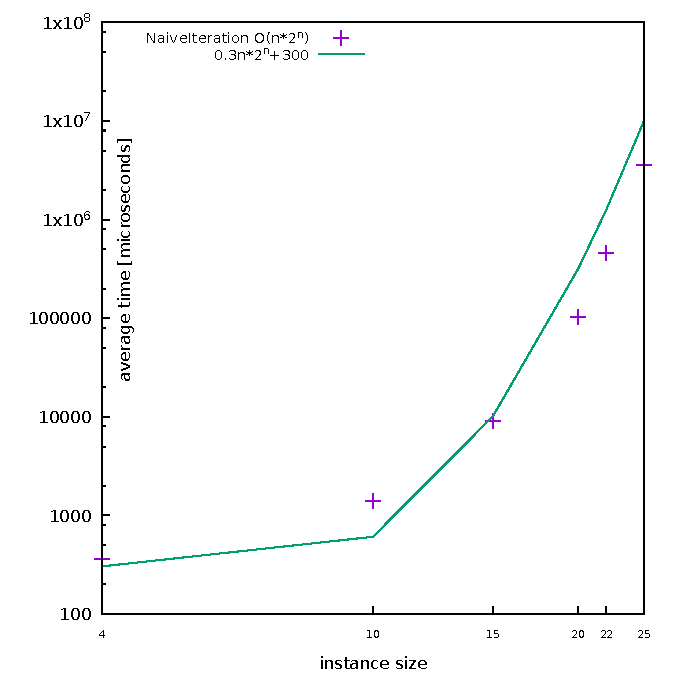
\includegraphics[width=9cm,height=9cm]{gnuplot/pdf/NaiveIteration.pdf}
  \end{center}
  \caption{NaiveIteration}\label{naiveIterationPlot}
\end{figure}

\subsection{Naive Recursion} \label{naiverec}
Another way to look at all the possible item combinations is a binary tree.
\begin{lstlisting}
1. The root represents an empty knapsack.
2. Right children at level i+1 include item i.
3. Left children at level i+1 do not include item i.
\end{lstlisting}
Traversing such tree makes it easy to keep track of the weight and value of given node. No significant computations are
required, which makes the worst case complexity the same as the number of nodes, $\mathcal{O}(2^n)$.

\begin{lstlisting}[frame=tlrb,language=scala,basicstyle=\scriptsize,label=naiveRecursionCode,caption=NaiveRecursion]
val items: Array[(Int, Int)] = ???
val capacity: Int = ???
var bestW, bestV = 0

def go(w: Int, v: Int, idx: Int): Unit = {
  if (w > capacity) return
  if (v > bestV) { bestV = v; bestW = bestW }
  if (idx == items.length) return
  go(w, v, idx + 1)
  go(w + items(idx).w, v + items(idx).v, idx + 1)
}
\end{lstlisting}

\begin{figure}[H]
  \begin{center}
        \hspace*{-1.2cm}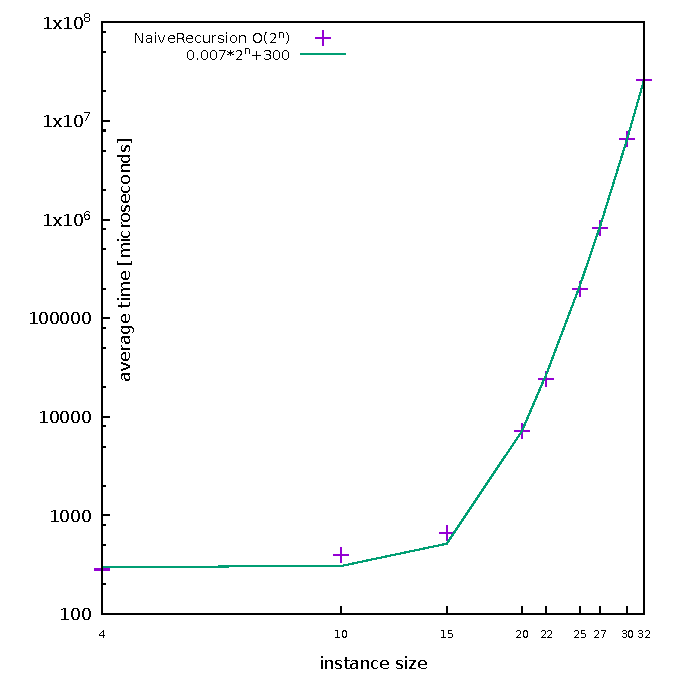
\includegraphics[width=9cm,height=9cm]{gnuplot/pdf/NaiveRecursion.pdf}
  \end{center}
  \caption{NaiveRecursion}\label{fig1}
\end{figure}

\subsection{BranchAndBound}
The Branch and bound method uses two strategies to reduce the number of traversed item combinations. Firstly it doesn't
explore branches where the weight is higher than the knapsack capacity, and secondly it doesn't explore branches where
the remaining items have lower total value than what would be needed to improve the best solution. The worse-case time
complexity is the same as with the recursive method, $\mathcal{O}(2^n)$.

\begin{lstlisting}[frame=tlrb,language=scala,basicstyle=\scriptsize,label=branchAndBoundCode,caption=BranchAndBound]
var best = Configuration.identity
val configIndices: mutable.BitSet = mutable.BitSet.empty
val idealValue: Int = items.map(_.v).sum

def go(skippedValue: Int, w: Int, v: Int, idx: Int): Unit = {
  if (best.value >= idealValue - skippedValue) return
  if (w > capacity) return
  if (v > best.value) best = Configuration(w, v, new mutable.BitSet(configIndices.toBitMask))
  if (idx == items.length) return

  go(skippedValue + items(idx).v, w, v, idx + 1)

  configIndices.add(idx)
  go(skippedValue, w + items(idx).w, v + items(idx).v, idx + 1)
  configIndices.remove(idx)
}
\end{lstlisting}

The first two parameters of the recursive function, $skippedValue$ and $w$, allow us to skip two kinds of branches:
Those whose remaining items aren't valuable enough to matter, and those that already exceed the knapsack
capacity.

\begin{figure}[H]
  \begin{center}
    \hspace*{-0.5cm}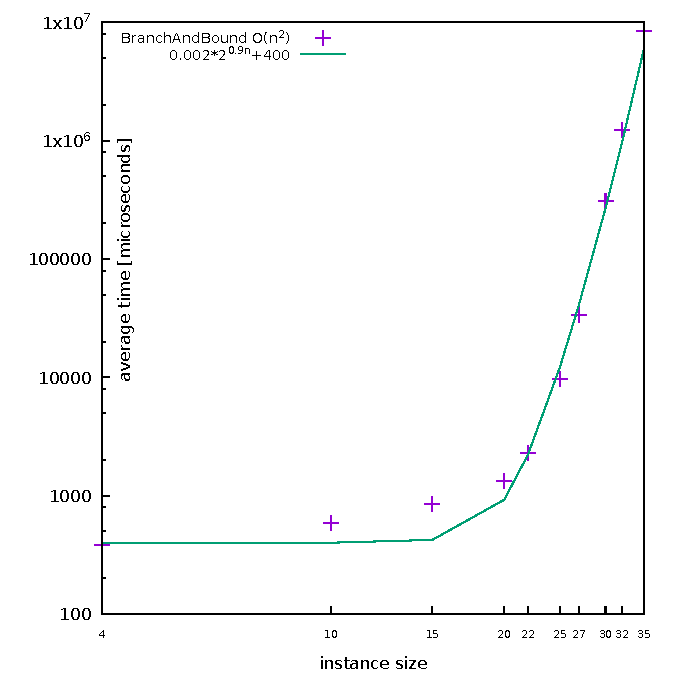
\includegraphics[width=9cm,height=9cm]{gnuplot/pdf/BranchAndBound.pdf}
  \end{center}
  \caption{Branch and bound}\label{fig1}
\end{figure}

The performance of this method was much faster than naive recursion using our test data, but it is highly dependent on
the instance parameters. If we had an instance whose last item is more valuable than the sum of all others, with
knapsack that can hold all the items, it would be just as slow as NaiveRecursion.

\subsection{DPByCapacity}
Dynamic programming, divides the problem into smaller problems with limited knapsack capacity. The tight bound
complexity is $\Theta(C \cdot n)$, where C is the capacity and n is the number of items. Complexity theory measures
difficulty with respect to the length of input, rather than its value, which is why we call the aforementioned
complexity pseudo-polynomial. It is exponential in the number of bits of $C$, but polynomial in the value of $C$. In
other words, the complexity is actually $\Theta(2^{C_b} \cdot n)$, where $C_b$ is the number of bits in $C$.

\begin{lstlisting}[frame=tlrb,language=scala,basicstyle=\scriptsize,label=dpByCapacityCode,caption=DPByCapacity]
for {
  col <- 0 to capacity
  row <- items.indices
  candidate = items(row)
} {
  if (row >= 1) {
    if (col >= candidate.w) {
      val withItem = solutions(row-1)(col-candidate.w) + candidate.v
      val withoutItem = solutions(row-1)(col)
      solutions(row)(col) = Math.max(withItem, withoutItem)
    } else solutions(row)(col) = solutions(row-1)(col)
  } else solutions(row)(col) = if (col < candidate.w) 0 else candidate.v
}
\end{lstlisting}

\begin{figure}[H]
  \begin{center}
    \hspace*{-0.5cm}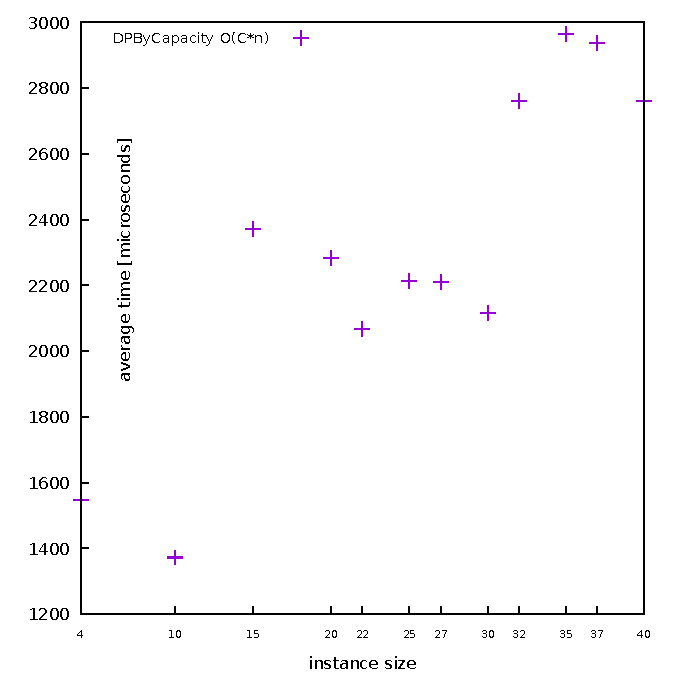
\includegraphics[width=9cm,height=9cm]{gnuplot/pdf/DPByCapacity.pdf}
  \end{center}
  \caption{DPByCapacity}\label{dpByCapacityPlot}
\end{figure}

\subsection{DPByValue}\label{DPByValue}
Dynamic programming divides a problem into smaller subproblems and stores their solutions in order not to solve the same
subproblem twice. As a result we often reduce exponential problems to polynomial complexity. The DPByValue algorithm
first solves a subproblem with just one item, then two, three and so on. Its $\Theta$ complexity is
$\Theta(T \cdot n)$, where $T$ is the sum of values of all items. Just like DPByCapacity, it runs in pseudo-polynomial
time.

\begin{lstlisting}[frame=tlrb,language=scala,basicstyle=\scriptsize,label=dpByValueCode,caption=DPByValue]
for {
  row <- 0 to totalValue
  col <- items.indices
  candidate = items(col)
} {
  val copy = if (col >= 1) solutions(row)(col-1) else 0
  val compose = candidate.v match {
    case v if col >= 1 && row > v => if (solutions(row - v)(col - 1) > 0) solutions(row - v)(col - 1) + candidate.w else 0
    case v if row == v => candidate.w
    case v => 0
  }

  solutions(row)(col) = if (copy != 0 && compose != 0) Math.min(copy, compose) else Math.max(copy, compose)
}
\end{lstlisting}

\begin{figure}[H]
  \begin{center}
    \hspace*{-0.5cm}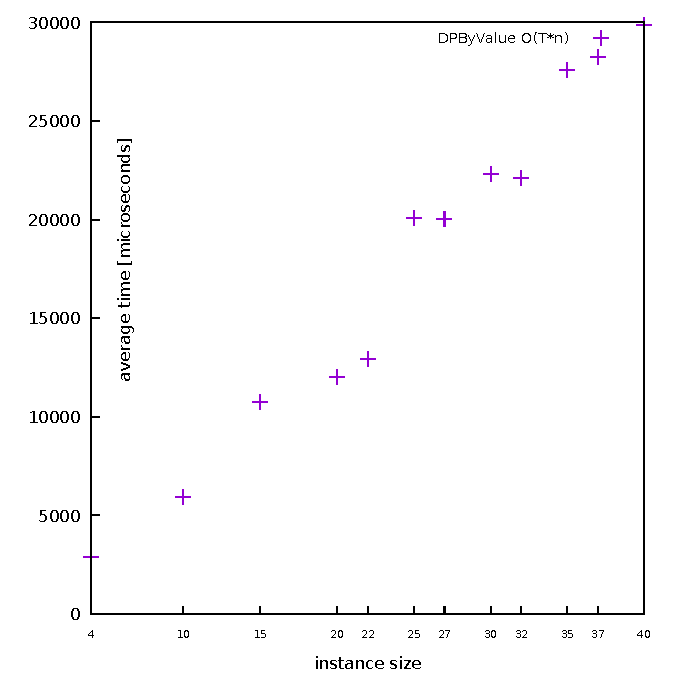
\includegraphics[width=9cm,height=9cm]{gnuplot/pdf/DPByValue.pdf}
  \end{center}
  \caption{DPByCapacity}\label{dpByCapacityPlot}
\end{figure}

\section{Approximative methods}
As the name suggests, approximative methods try to find near-optimal solutions. The following formula was used to
calculate the relative error of a signle solution: \\

$\varepsilon = \frac{V(OPT)-V(APX)}{V(OPT)}$ \\

Where $V(OPT)$ is the value of the optimal solution and $V(APX)$ is the value of the approximated solution.

\subsection{Value/Weight Ratio Heuristic}
The following algorithm has the asymptotic computational complexity of the sorting algorithm it uses,
which is $\mathcal{O}(n\log{n})$ in our case.

\begin{lstlisting}[frame=tlrb,language=scala,basicstyle=\scriptsize,label=vwRatioHeuristicCode,caption=VWRatioHeuristic]
var accW, accV = 0
val sorted = items.sortWith((l, r) => (l.v / l.w) > (r.v / r.w))
sorted foreach { itm =>
  if (accW + itm.w <= capacity) {
    accW += itm.w
    accV += itm.v
  }
}
\end{lstlisting}

The heuristic is very straightforward and yields surprisingly accurate results, see figure \ref{vwratioavgerr}. On the
other hand, it does not guarantee high accuracy. Suppose we have a knapsack that can carry 100 weight units and the
following items: {(w:51,v:34),(w:50,v:33),(w:50,v:33)}. VWRatioHeuristic will happily fill the knapsack with the first
item, achieving the total value of 34. The optimal solution would use the two other items, achieving the value of 66. It
is apparent that the worst-case relative error is close to 50\%.

\begin{figure}[H]
  \begin{center}
    \hspace*{-0.5cm}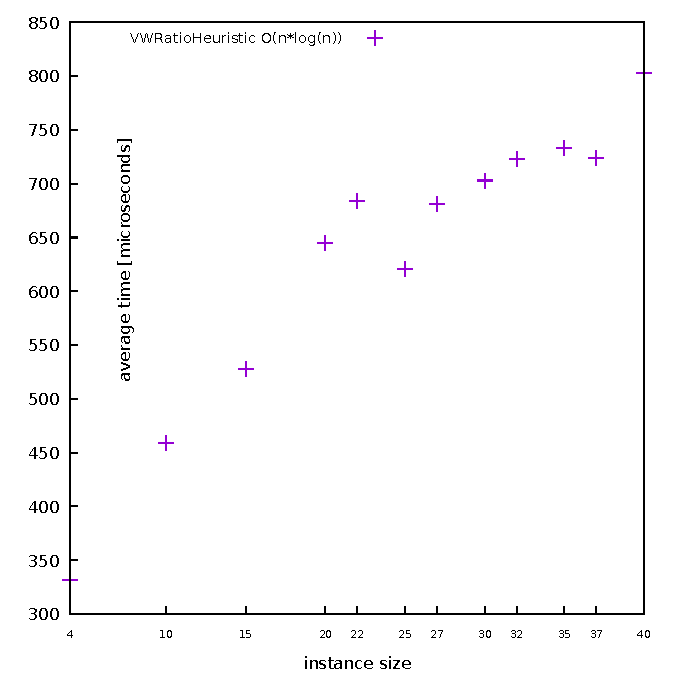
\includegraphics[width=9cm,height=9cm]{gnuplot/pdf/VWRatioHeuristic.pdf}
  \end{center}
  \caption{VWRatioHeuristic}\label{vwRatioHeuristicPlot}
\end{figure}

The following tables show the average and maximum relative errors of the VWRatioHeuristic algorithm.

\begin{figure}[H]
    \begin{lstlisting}[basicstyle=\scriptsize]
    n     4      10      15      20     22      25      30     35    40
    avgE  1.94%  1.43%   .49%    .54%   .69%    .72%    .72%   .50%  .53%
    \end{lstlisting}
    \caption{Average error of the V/W ratio heuristic.}\label{vwratioavgerr}
\end{figure}

\begin{figure}[H]
    \begin{lstlisting}[basicstyle=\scriptsize]
    n      4      10     15     20     22     25      30     35     40
    maxE   24.7%  11.5%  8.54%  8.43%  7.23%  3.68%   5.51%  4.60%  2.34%
    \end{lstlisting}
    \caption{Maximal error of the V/W ratio heuristic.}\label{vwratiomaxerr}
\end{figure}

As we can see, the heuristic was fairly successful at finding near-optimal solutions and its precision increases with
the number of items.

\subsection{FPTAS}
The acronym FPTAS stands for Fully Polynomial-time Approximation Scheme. In general, an approximation scheme trades
accuracy for efficiency. How would we go about it in context of the Knapsack problem?

So far we've demonstrated two algorithms whose complexity is dependent on other variables than the item count $n$.
DPByCapacity was also dependent on the capacity of the knapsack, and DPByValue was dependent on the sum of item values.

What would happen if we divided all the item values by 2 and rounded them to the nearest integer? The sum of item
values, $T$, would be halved, reducing running time by $2n$, because the complexity is $\Theta(T \cdot n)$.

If we somehow managed to bound $T$ by a power of $n$, we'd have truly polynomial complexity. It is possible. Actually
all we have to do is to divide $T$ by the value of the most valuable item, $VMax$:

$$T_{B} = \frac{T}{VMax} = \frac{\sum_{i=1}^{n} item[i].v}{VMax} <= \frac{n \cdot VMax}{VMax} = n$$

By preprocessing input in this way, we can get polynomial running time for the DPByValue algorithm:

$\Theta(T_{B} \cdot n) = \Theta(n^2)$, where $T_B$ is sum of the values of prepreocessed items.

So far we didn't take accuracy into account, and reducing the sum of item values to $n$ means that the average item
value is $<= 1$. We can fix this by dividing $VMax$ by $\frac{1}{\varepsilon} n$. Consequently the average item will have the
value of $\frac{1}{\varepsilon} n$ and the complexity will be $\Theta(\frac{n^3}{\varepsilon})$

\begin{figure}[H]
  \begin{center}
    \hspace*{-0.5cm}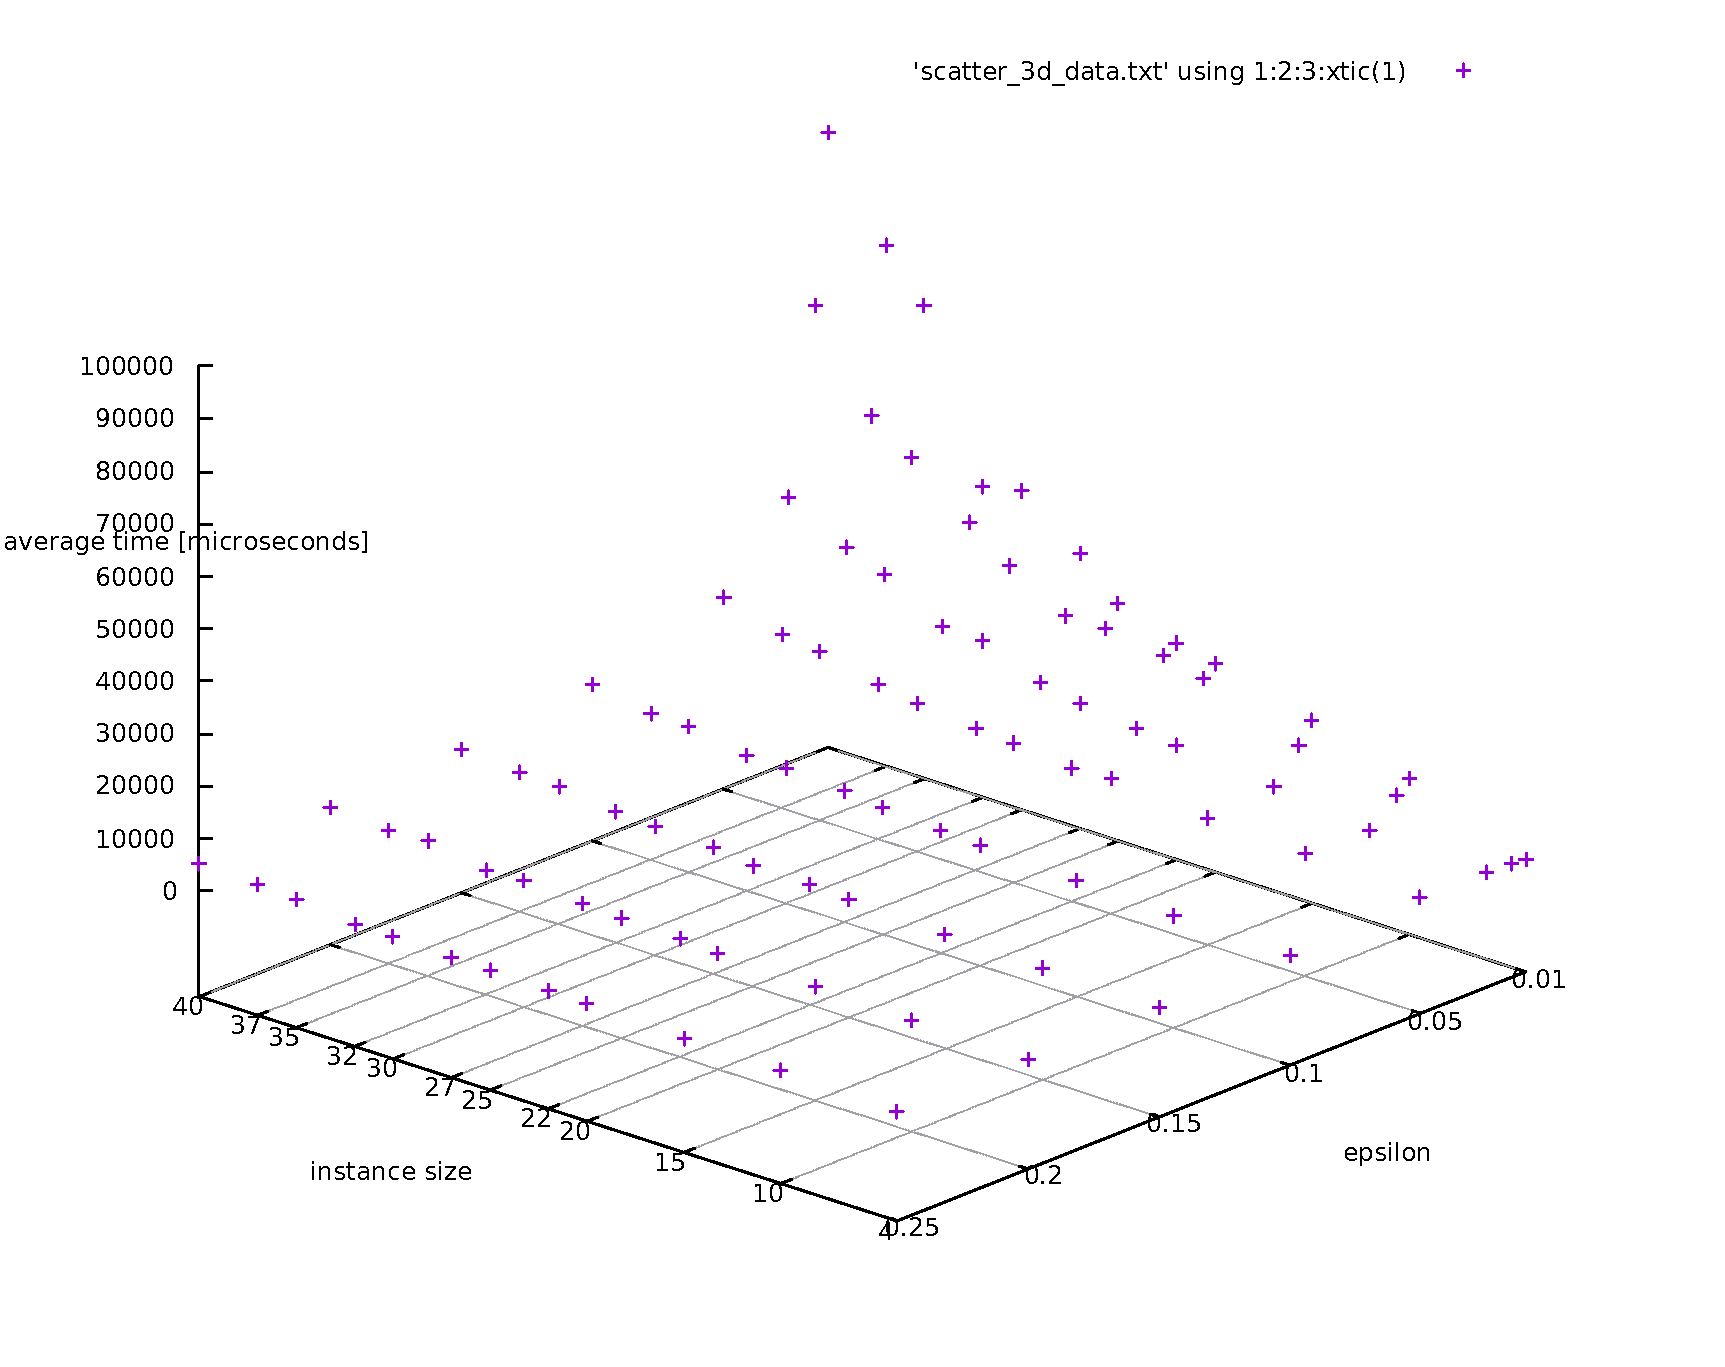
\includegraphics[width=9cm,height=9cm]{gnuplot/pdf/FPTAS_splot.pdf}
  \end{center}
  \caption{FPTAS}\label{fptasPlot}
\end{figure}

\paragraph{Conclusion} We have implemented and demonstrated a polynomial class algorithm that solves the knapsack
problem with arbitrary accuracy. In other words, we have implemented a fully polynomial approximation scheme for the
knapsack problem.

\section{Implementation} % popis kostry algoritmu (nikoliv výpis kódu!)
I chose Scala as the implementation language for its simplicity. See scaladoc comments in the code for implementation
details.

The project is structured into classes. Different algorithms are in separate files in the $solvers$ package, e.g.
solvers/NaiveIteration.scala.

\section{Conclusion} % závěr: interpretace výsledků a zdůvodnění jejich kvality
The Naive Iteration algorithm turned out to perform much worse than recursion. On the other hand, the recursive
algorithm and the heuristic performed to our expectations in regard to computational complexity.

The value/weight ratio heuristic yielded surprisingly good results, within 2\% of the optimal solutions. Other methods,
such as simulated evolution, may give even better approximations with little increase in time complexity.

\begin{thebibliography}{9}
    \bibitem{wikiKnapsack}
        Knapsack problem.
        In: \textit {Wikipedia} [online].
        [vid. 12.10.2016]. Available at:
        \url{https://en.wikipedia.org/wiki/Knapsack_problem}
\end{thebibliography}

\end{document}